\ifdefined\maindoc\else
% typesetting this chapter as a standalone document
\def\doctitle{Fields}
% starting definitions for both the main document and stand-alone chapters
\documentclass{book}

\def\mech{artisynth.core.mechmodels}
\def\mgeo{maspack.geometry}

% Add search paths for input files
\makeatletter
\def\input@path{{../}{../../}{../texinputs/}}
\makeatother

\usepackage{amsmath}
\usepackage{framed}
%%
%% Default settings for artisynth
%%
\NeedsTeXFormat{LaTeX2e}
%%\ProvidesPackage{artisynthDoc}[2012/04/05]

\usepackage[T1]{fontenc}
\usepackage[latin1]{inputenc}
\usepackage{listings}
\usepackage{makeidx}
\usepackage{latexml}
\usepackage{graphicx}
\usepackage{framed}
\usepackage{booktabs}
\usepackage{color}

\newcommand{\pubdate}{\today}
\newcommand{\setpubdate}[1]{\renewcommand{\pubdate}{#1}}
\newcommand{\code}[1]{{\tt #1}}

\iflatexml
\usepackage{hyperref}
\setlength\parindent{0pt} 
\else
%% then we are making a PDF, so include things that LaTeXML can't handle: 
%% docbook style, \RaggedRight
\usepackage{ifxetex}
\usepackage{xstring}
\usepackage{pslatex} % fixes fonts; in particular sets a better-fitting \tt font

\usepackage[most]{tcolorbox}
\definecolor{shadecolor}{rgb}{0.95,0.95,0.95}
\tcbset{
    frame code={}
    center title,
    left=0pt,
    right=0pt,
    top=0pt,
    bottom=0pt,
    colback=shadecolor,
    colframe=white,
    width=\dimexpr\textwidth\relax,
    enlarge left by=0mm,
    boxsep=0pt,
    arc=0pt,outer arc=0pt,
}%

\usepackage[A4]{artisynth_papersize}
%\usepackage[letter]{artisynth_papersize}
\usepackage[hyperlink]{asciidoc-dblatex} 

%\usepackage{verbatim}
\usepackage{ragged2e}
\setlength{\RaggedRightRightskip}{0pt plus 4em}
\RaggedRight
\renewcommand{\DBKpubdate}{\pubdate}
\renewcommand{\DBKreleaseinfo}{}
\fi

% set hypertext links to be dark blue:
\definecolor{darkblue}{rgb}{0,0,0.8}
\definecolor{sidebar}{rgb}{0.5,0.5,0.7}
\hypersetup{colorlinks=true,urlcolor=darkblue,linkcolor=darkblue,breaklinks=true}

%%%%%%%%%%%%%%%%%%%%%%%%%%%%%%%%%%%%%%%%%%%%%%%%%%%%%%%%%%%%%%%%%%%%%%%%%%%%%
%
% Define macros for handling javadoc class and method references
%
%%%%%%%%%%%%%%%%%%%%%%%%%%%%%%%%%%%%%%%%%%%%%%%%%%%%%%%%%%%%%%%%%%%%%%%%%%%%%
\makeatletter

% macro to enable line break if inside a PDF file
\def\pdfbreak{\iflatexml\else\\\fi}

% code inspired by http://stackoverflow.com/questions/2457780/latex-apply-an-operation-to-every-character-in-a-string
\def\removeargs #1{\doremoveargs#1$\wholeString\unskip}
\def\doremoveargs#1#2\wholeString{\if#1$%
\else\if#1({()}\else{#1}\taketherest#2\fi\fi}
\def\taketherest#1\fi
{\fi \doremoveargs#1\wholeString}

% Note: still doesn't work properly when called on macro output ...
% i.e., \dottoslash{\concatnames{model}{base}{foo}} fails 
\def\dottoslash #1{\dodottoslash#1$\wholeString\unskip}
\def\dodottoslash#1#2\wholeString{\if#1$%
\else\if#1.{/}\else{#1}\fi\dottaketherest#2\fi}
\def\dottaketherest#1\fi{\fi \dodottoslash#1\wholeString}

\def\hashtodot #1{\dohashtodot#1$\wholeString\unskip}
\def\dohashtodot#1#2\wholeString{\if#1$X%
\else\if#1\#{.}\else{#1}\fi\hashtaketherest#2\fi}
\def\hashtaketherest#1\fi{\fi \dohashtodot#1\wholeString}

%\dollartodot{#1} does the same thing as \StrSubstitute[0]{#1}{\$}{.}
% from the packahe xstring. We define \dollartodot instead because
% LaTeXML does not implement xstring.
%
% Note that for the substituion to work, we need \ifx instead of \if,
% since otherwise escaped characters won't work properly:
% if #1 = \$, then \if#1* seems to compare '\' and '$' (and output '*'),
% rather than comparing '$' to '*'
\def\dollartodot #1{\dodollartodot#1*\wholeString\unskip}
\def\dodollartodot#1#2\wholeString{\ifx#1*%
\else \ifx#1\${.}\else{#1}\fi\dollartaketherest#2\fi}
\def\dollartaketherest#1\fi{\fi \dodollartodot#1\wholeString}

% concatenates up to three class/method names together, adding '.' characters
% between them. The first and/or second argument may be empty, in which case
% the '.' is omitted. To check to see if these arguments are empty, we
% use a contruction '\if#1@@', which will return true iff #1 is empty
% (on the assumption that #1 will not contain a '@' character).
\def\concatnames
#1#2#3{\if#1@@\if#2@@#3\else #2.#3\fi\else\if#2@@#1.#3\else#1.#2.#3\fi\fi}

\newcommand{\javabase}{}
\newcommand{\setjavabase}[1]{\renewcommand{\javabase}{#1}}

\def\artisynthDocBase{@ARTISYNTHDOCBASE}

\iflatexml
\def\ifempty#1{\def\temp{#1}\ifx\temp\empty}%
\newcommand{\artisynthManual}[3][]{%
   \ifempty{#1}
      \href{@ARTISYNTHDOCBASE/#2/#2.html}{#3}%
    \else
      \href{@ARTISYNTHDOCBASE/#1/#2.html}{#3}%
    \fi
}
\else
\newcommand{\artisynthManual}[3][]{%
\href{https://www.artisynth.org/@ARTISYNTHDOCBASE/#2.pdf}{#3}}
\fi

%\href{@ARTISYNTHDOCBASE/#2/#2.html}{#3}}



\newcommand{\javaclassx}[2][]{%
% Includes code to prevent an extra '.' at the front if #1 is empty. It
% works like this: if '#1' is empty, then '#1.' expands to '.', and so 
% '\if#1..' will return true, in which case we just output '#2'.
\href{@JDOCBEGIN/\concatnames{\javabase}{#1}{#2}@JDOCEND}{#2}}
\newcommand{\javaclass}[2][]{%
\href{@JDOCBEGIN/\concatnames{}{#1}{#2}@JDOCEND}{\dollartodot{#2}}}
\newcommand{\javaclassAlt}[2]{%
\href{@JDOCBEGIN/\concatnames{}{}{#1}@JDOCEND}{#2}}

\newcommand{\javamethodArgsx}[2][]{%
\href{@JDOCBEGIN/\concatnames{\javabase}{#1}{#2}@JDOCEND}{#2}}
\newcommand{\javamethodArgs}[2][]{%
\href{@JDOCBEGIN/\concatnames{}{#1}{#2}@JDOCEND}{#2}}
\newcommand{\javamethodAlt}[2]{%
\href{@JDOCBEGIN/\concatnames{}{}{#1}@JDOCEND}{#2}}
\newcommand{\javamethodAltx}[2]{%
\href{@JDOCBEGIN/\concatnames{\javabase}{}{#1}@JDOCEND}{#2}}

\newcommand{\javamethodNoArgsx}[2][]{%
\href{@JDOCBEGIN/\concatnames{\javabase}{#1}{#2}@JDOCEND}{\removeargs{#2}}}
\newcommand{\javamethodNoArgs}[2][]{%
\href{@JDOCBEGIN/\concatnames{}{#1}{#2}@JDOCEND}{\removeargs{#2}}}

\newcommand{\javamethod}{\@ifstar\javamethodNoArgs\javamethodArgs}
\newcommand{\javamethodx}{\@ifstar\javamethodNoArgsx\javamethodArgsx}

%%%%%%%%%%%%%%%%%%%%%%%%%%%%%%%%%%%%%%%%%%%%%%%%%%%%%%%%%%%%%%%%%%%%%%%%%%%%%
%
% Define macros for sidebars
%
%%%%%%%%%%%%%%%%%%%%%%%%%%%%%%%%%%%%%%%%%%%%%%%%%%%%%%%%%%%%%%%%%%%%%%%%%%%%%

\iflatexml
\newenvironment{sideblock}{\begin{quote}}{\end{quote}}
\else
\usepackage[strict]{changepage}
\definecolor{sidebarshade}{rgb}{1.0,0.97,0.8}
\newenvironment{sideblock}{%
    \def\FrameCommand{%
    \hspace{1pt}%
    {\color{sidebar}\vrule width 2pt}%
    %{\vrule width 2pt}%
    {\color{sidebarshade}\vrule width 4pt}%
    \colorbox{sidebarshade}%
  }%
  \MakeFramed{\advance\hsize-\width\FrameRestore}%
  \noindent\hspace{-4.55pt}% disable indenting first paragraph
  \begin{adjustwidth}{}{7pt}%
  %\vspace{2pt}\vspace{2pt}%
}
{%
  \vspace{2pt}\end{adjustwidth}\endMakeFramed%
}
\fi

\iflatexml
\newenvironment{shadedregion}{%
  \definecolor{shadecolor}{rgb}{0.96,0.96,0.98}%
  \begin{shaded*}%
% Put text inside a quote to create a surrounding blockquote that
% will properly accept the color and padding attributes
  \begin{quote}%
}
{%
  \end{quote}%
  \end{shaded*}%
}
\else
\newenvironment{shadedregion}{%
  \definecolor{shadecolor}{rgb}{0.96,0.96,0.98}%
  \begin{shaded*}%
}
{%
  \end{shaded*}%
}
\fi

% Wanted to create a 'listing' environment because lstlisting is
% tedious to type and because under latexml it may need
% some massaging to get it to work properly. But hard to do
% because of the verbatim nature of listing
%\iflatexml
%\newenvironment{listing}{\begin{lstlisting}}{\end{lstlisting}}%
%\else
%\newenvironment{listing}{\begin{lstlisting}}{\end{lstlisting}}%
%\fi

\iflatexml\else
% fancyhdr was complaining that it wanted a 36pt header height ...
\setlength{\headheight}{36pt}
\fi

% macro for backslash character
\newcommand\BKS{\textbackslash}

% macro for double hyphen (to prevent conversion of -- into -)
\newcommand\DHY{-{}-}

% Convenience stuff
\newcommand{\ifLaTeXMLelse}[2]{%
  \iflatexml %
  #1 %
  \else %
  #2 %
  \fi %
}

\newcommand{\ifLaTeXML}[1]{ %
  \iflatexml %
  #1 %
  \fi %
}

% new methodtable environment for documenting methods

% base width of the method table
\newlength{\methodtablewidth}
\iflatexml
\setlength{\methodtablewidth}{1.4\textwidth}
\else
\setlength{\methodtablewidth}{0.94\textwidth}
\fi
% horizontal space added at end of call to \methodentry
\newlength{\methodskip}
\setlength{\methodskip}{0pt}
% lengths set inside methodtable environment:
\newlength{\methodsiglength} % length of the method signature
\newlength{\methodcomlength} % length of the method comment
\setlength{\methodsiglength}{0.5\methodtablewidth}
\setlength{\methodcomlength}{0.5\methodtablewidth}

% command to add a method to a method table:
% arg #1: package and signature for finding URL
% arg #2: anchor text
% arg #3: comment describing the method
\newcommand{\methodentry}[3]{%
\javamethodAlt{#1}{\parbox[t]{\methodsiglength}{#2}}&
{\parbox[t]{\methodcomlength}{#3}}\\%
\noalign{\vspace{\methodskip}}}

% methodtable environment takes two arguments, both scale factors for
% methodtablewidth:
% arg #1: width of the method signature column
% arg #2: width of the method comment column
\newenvironment{methodtable}[3][0pt]{%
\begingroup
\setlength{\topskip}{0pt}
\setlength{\methodskip}{#1}
\setlength{\methodsiglength}{#2\methodtablewidth}%
\setlength{\methodcomlength}{#3\methodtablewidth}%
\iflatexml
\begin{snugshade}
\else
\begin{tcolorbox}
\fi
\renewcommand{\arraystretch}{1}
\begin{tabular}{ll}}{%
\end{tabular}
\renewcommand{\arraystretch}{1}
\iflatexml
\end{snugshade}
\else
\end{tcolorbox}
\fi
\endgroup}

% commands for added top, mid and bottom lines in the table.
% uses booktabs for PDF, regular hline for HTML
\newcommand{\topline}{\iflatexml\hline\else\toprule\fi}
\newcommand{\midline}{\iflatexml\hline\else\midrule\fi}
\newcommand{\botline}{\iflatexml\hline\else\bottomrule\fi}
\newcommand{\blankline}{%
\multicolumn{2}{l}{\iflatexml{@SPACE}\else\phantom{M}\fi}\\}%
% add vertical space within a two colum method environment
\newcommand{\methodspace}[1]{%
\iflatexml
\multicolumn{2}{l}{@VERTSPACE[#1]}\\
\else
\noalign{\vspace{#1}}%
\fi}%
% break a line and add an indentation of 1em
\newcommand{\brh}{\\\phantom{M}}

\makeatother

\def\matl{\left(\begin{matrix}}
\def\matr{\end{matrix}\right)}

\def\Bthe{\boldsymbol\theta}
\def\Btau{\boldsymbol\tau}
\def\Bom{\boldsymbol\omega}
\def\Bdel{\boldsymbol\delta}
\def\Blam{\boldsymbol\lambda}
\def\Bphi{\boldsymbol\phi}
\def\Bxi{\boldsymbol\xi}
\def\Bgam{\boldsymbol\gamma}
\def\Bsig{\boldsymbol\sigma}
\def\Bnu{\boldsymbol\nu}
\def\Bmu{\boldsymbol\mu}

\def\A{{\bf A}}
\def\B{{\bf B}}
\def\C{{\bf C}}
\def\D{{\bf D}}
\def\F{{\bf F}}
\def\G{{\bf G}}
\def\H{{\bf H}}
\def\I{{\bf I}}
\def\J{{\bf J}}
\def\K{{\bf K}}
\def\Jc{{\bf J}_c}
\def\L{{\bf L}}
\def\M{{\bf M}}
\def\N{{\bf N}}
\def\O{{\bf O}}
\def\P{{\bf P}}
\def\Q{{\bf Q}}
\def\R{{\bf R}}
\def\T{{\bf T}}
\def\U{{\bf U}}
\def\W{{\bf W}}
\def\X{{\bf X}}
\def\Minv{{\bf M}^{-1}}

\def\a{{\bf a}}
\def\b{{\bf b}}
\def\c{{\bf c}}
\def\d{{\bf d}}
\def\e{{\bf e}}
\def\f{{\bf f}}
\def\g{{\bf g}}
\def\k{{\bf k}}
\def\l{{\bf l}}
\def\m{{\bf m}}
\def\n{{\bf n}}
\def\p{{\bf p}}
\def\q{{\bf q}}
\def\r{{\bf r}}
\def\u{{\bf u}}
\def\v{{\bf v}}
\def\w{{\bf w}}
\def\x{{\bf x}}
\def\y{{\bf y}}
\def\z{{\bf z}}

\def\ma{{\bf m}_\alpha}
\def\mb{{\bf m}_\beta}
\def\va{{\bf v}_\alpha}
\def\vb{{\bf v}_\beta}
\def\vp{{\bf v}_\rho}
\def\vk{{\bf v}_k}
\def\ua{{\bf u}_\alpha}
\def\ub{{\bf u}_\beta}
\def\uk{{\bf u}_k}
\def\uj{{\bf u}_j}
\def\mar{{\bf m}_{\alpha r}}
\def\mbr{{\bf m}_{\beta r}}

\def\Maa{{\bf M}_{\alpha\alpha}}
\def\Mab{{\bf M}_{\alpha\beta}}
\def\Mba{{\bf M}_{\beta\alpha}}
\def\Mbb{{\bf M}_{\beta\beta}}
\def\hatMaa{\hat{\bf M}_{\alpha\alpha}}
\def\hatMab{\hat{\bf M}_{\alpha\beta}}
\def\hatMba{\hat{\bf M}_{\beta\alpha}}
\def\hatMbb{\hat{\bf M}_{\beta\beta}}
\def\Mbp{{\bf M}_{\beta\rho}}
\def\Map{{\bf M}_{\alpha\rho}}
\def\Mpa{{\bf M}_{\rho\alpha}}
\def\Mpb{{\bf M}_{\rho\beta}}
\def\Mpp{{\bf M}_{\rho\rho}}
\def\Mbk{{\bf M}_{\beta k}}
\def\Mak{{\bf M}_{\alpha k}}
\def\Mka{{\bf M}_{k\alpha}}
\def\Mkb{{\bf M}_{k\beta}}
\def\Mkk{{\bf M}_{kk}}

\def\Ga{{\bf G}_{\alpha}}
\def\Gp{{\bf G}_{\rho}}
\def\Gaa{{\bf G}_{\alpha\alpha}}
\def\Gab{{\bf G}_{\alpha\beta}}
\def\Gba{{\bf G}_{\beta\alpha}}
\def\Gbb{{\bf G}_{\beta\beta}}
\def\Gap{{\bf G}_{\alpha\rho}}
\def\Gpa{{\bf G}_{\rho\alpha}}
\def\Gbp{{\bf G}_{\beta\rho}}
\def\Gak{{\bf G}_{\alpha k}}
\def\Gka{{\bf G}_{k\alpha}}
\def\Gja{{\bf G}_{j\alpha}}
\def\Gkb{{\bf G}_{k\beta}}
\def\Gbk{{\bf G}_{\beta k}}

\def\lama{\Blam_{\alpha}}
\def\lamb{\Blam_{\beta}}
\def\lamp{\Blam_{\rho}}
\def\lamk{\Blam_{k}}
\def\lams{\Blam_{\sigma}}

\def\ba{{\bf b}_{\alpha}}
\def\bb{{\bf b}_{\beta}}
\def\fp{{\bf f}_{\rho}}
\def\fa{{\bf f}_{\alpha}}
\def\qa{{\bf q}_{\alpha}}
\def\qb{{\bf q}_{\beta}}
\def\za{{\bf z}_{\alpha}}
\def\zb{{\bf z}_{\beta}}
\def\wa{{\bf w}_{\alpha}}
\def\wb{{\bf w}_{\beta}}

\def\Na{\bar{\bf N}_{\alpha}}
\def\Nb{\bar{\bf N}_{\beta}}

\def\Up{{\bf U}_p}
\def\Un{{\bf U}_n}

\def\dFdl{\frac{\partial F}{\partial l}}
\def\dFddl{\frac{\partial F}{\partial \dot l}}

\def\Sr{s_\theta}
\def\Cr{c_\theta}
\def\Sp{s_\phi}
\def\Cp{c_\phi}
\def\Sy{s_\psi}
\def\Cy{c_\psi}
\def\Sa{s_{\alpha}}
\def\Ca{c_{\alpha}}
\def\Vp{v_{\phi}}


\iflatexml
\else
\usepackage{biblatex}
\addbibresource{references.bib}
\fi

\setcounter{tocdepth}{5}
\setcounter{secnumdepth}{3}

\title{\doctitle}
\ifdefined\maindoc
\author{John Lloyd and Antonio S\'anchez}
\setpubdate{Last update: March, 2022}

\iflatexml
\date{}
\fi
\fi

% graphics paths
\graphicspath{{./}{images/}}

% Listings settings
\definecolor{myblue}{rgb}{0,0,0.6}
\definecolor{mygreen}{rgb}{0,0.6,0}
\definecolor{mygray}{rgb}{0.5,0.5,0.5}
\definecolor{mylightgray}{rgb}{0.95,0.95,0.95}
\definecolor{mymauve}{rgb}{0.58,0,0.82}
\definecolor{myblack}{rgb}{0,0,0}
\lstset{
   language=Java,                   % text highlighting for Java
   breakatwhitespace=false,         % automatic breaks only at whitespace
   breaklines=true,                 % automatic line breaking
   commentstyle=\color{mygreen},    % comment style
   keepspaces=true,                 % keeps spaces in text
   keywordstyle=\color{myblue},     % keyword style
   numbers=none,                    % line-numbers; values: (none, left, right)
   numbersep=5pt,                   % how far the line-numbers are from code
   numberstyle=\tiny\color{mygray}, % line-numbers style
   showspaces=false,                % show spaces everywhere
   showstringspaces=false,          % underline spaces within strings
   showtabs=false,                  % show tabs
   stepnumber=1,                    % the step between two line-numbers
   stringstyle=\color{mymauve},     % string literal style
   tabsize=3,                       % sets default tabsize to 3 spaces
   backgroundcolor=\color{mylightgray}, % background color
   frame=single, 					% adds a frame around the code
   rulesepcolor=\color{mygray},
   rulecolor=\color{myblack},
   framerule=0pt,
   xleftmargin=2.2ex,               % numbers inside box
   framexleftmargin=2.2ex,			% indentation of frame
}

\begin{document}

\frontmatter

%\layout
\maketitle

\iflatexml{\large\pubdate}\fi

\tableofcontents

\mainmatter
\fi

\chapter{Fields}
\label{sec:fields}

In modeling applications, particularly those employing FEM methods,
situations often arise where it is necessary to describe numeric
quantities that vary over some spatial domain. For example, the
stiffness parameters of an FEM material may vary at different points
within the volumetric mesh.  When modeling muscles, the activation
direction vector will also typically vary over the mesh.

ArtiSynth provides {\it field components} which can be used to
represent such spatially varying quantities, together with mechanisms
to attach these to certain properties within various materials.  Field
components can implement either {\it scalar} or {\it vector}
fields. Scalar field components implement the interface
\javaclass[artisynth.core.modelbase]{ScalarFieldComponent} and supply
the method
%
\begin{lstlisting}[]
   double getValue (Point3d p)
\end{lstlisting}
%
while vector fields implement
\javaclass[artisynth.core.modelbase]{VectorFieldComponent}
and supply the method
%
\begin{lstlisting}[]
   T getValue (Point3d p)
\end{lstlisting}
%
where {\tt T} parameterizes a class implementing
\javaclass{maspack.matrix.VectorObject}.  In both cases, the idea is
to provide values at arbitrary points over some spatial domain.

For vector fields, the {\tt VectorObject} represented by {\tt T} can
generally be any {\it fixed-size} vector or matrix located in the
package {\tt maspack.matrix}, such as
\javaclass[maspack.matrix]{Vector2d},
\javaclass[maspack.matrix]{Vector3d}, or
\javaclass[maspack.matrix]{Matrix3d}. {\tt T} can {\it also} be one of
the variable-sized objects \javaclass[maspack.matrix]{VectorNd} or
\javaclass[maspack.matrix]{MatrixNd}, although this requires using
special wrapper classes and the sizing must remain constant within the
field (Section \ref{sec:wrapperFields}).

\begin{sideblock}
Both {\tt ScalarFieldComponent} and {\tt VectorFieldComponent} are
subclassed from {\tt FieldComponent}. The reason for separating scalar
and vector fields is simply efficiency: having scalar fields work with
the primitive type {\tt double}, instead of the object {\tt Double},
requires considerably less storage and somewhat less computational
effort.
\end{sideblock}

A field is typically implemented by specifying a finite set of values
at discrete locations on an underlying spatial grid and then using an
interpolation method to determine values at arbitrary points. The
field components themselves are defined within the package {\tt
artisynth.core.fields}.

At present, three types of fields are implemented:

\begin{description}

\item[Grid fields]\mbox{}

The most basic type of field, in which the values are specified at the
vertices of a regular Cartesian grid and then interpolated between
vertices. As discussed further in Section \ref{sec:gridFields}, there
are two main types grid field component:
\javaclass[artisynth.core.fields]{ScalarGridField} and
\javaclassAlt{artisynth.core.fields.VectorGridField}{VectorGridField<T>}.

\item[FEM fields]\mbox{}

Fields for which values are specified at the features of an FEM mesh
(e.g., nodes, elements or element integration points).  As discussed
further in Section \ref{sec:femFields}, there are six primary types of
FEM field component:
\javaclass[artisynth.core.fields]{ScalarNodalField}
and
\javaclassAlt{artisynth.core.fields.VectorNodalField}{VectorNodalField<T>}
(nodes),
\javaclass[artisynth.core.fields]{ScalarElementField}
and
\javaclassAlt{artisynth.core.fields.VectorElementField}{VectorElementField<T>}
(elements), and
\javaclass[artisynth.core.fields]{ScalarSubElemField}
and
\javaclassAlt{artisynth.core.fields.VectorSubElemField}{VectorSubElemField<T>}
(integration points).

\item[Mesh fields]\mbox{}

Fields in which values are specified for either the vertices or faces
of a triangular mesh. As discussed
further in Section \ref{sec:meshFields}, there are four primary types of
mesh field component:
\javaclass[artisynth.core.fields]{ScalarVertexField}
and
\javaclassAlt{artisynth.core.fields.VectorVertexField}{VectorVertexField<T>}
(vertices), and 
\javaclass[artisynth.core.fields]{ScalarFaceField}
and
\javaclassAlt{artisynth.core.fields.VectorFaceField}{VectorFaceField<T>}
(faces).

\end{description}

Within an application model, field deployment typically involves the
following steps:

\begin{enumerate}

\item Create the field component and add it to the model. Grid and
mesh fields are usually added to the {\it fields} component list of a
\javaclass[artisynth.core.mechmodels]{MechModel}, while FEM fields are
added to the {\it fields} list of the
\javaclass[artisynth.core.femmodels]{FemModel3d} for which the field
is defined.

\item Specify field values for the appropriate features (e.g.,
grid vertices, FEM nodes, mesh faces).

\item If necessary, bind any needed material properties
to the field, as discussed further in Section \ref{sec:fieldBinding}.

\end{enumerate}

As a simple example of the first two steps, the following code
fragment constructs a scalar nodal field associated with an FEM model
named {\tt fem}:
%
\begin{lstlisting}[]
   FemModel3d fem; 
   // ... build the fem ...
   ScalarNodalField field = new ScalarNodalField ("stiffness", fem, 0);
   for (FemNode3d n : fem.getNodes()) {
      double value = ... // compute value for the node
      field.setValue (n, value);
   }
   fem.addField (field); // add the field to the fem
\end{lstlisting}
%

More details on specific field components are given in the sections
below.

\section{Grid fields}
\label{sec:gridFields}

A grid field specifies scalar or vector values at the vertices of a
regular Cartesian grid and interpolates values between vertices.
ArtiSynth currently provides two grid field components in {\tt
artisynth.core.fields}:
%
\begin{lstlisting}[]
   ScalarGridField

   VectorGridField<T>
\end{lstlisting}
%
where {\tt T} is any class implementing
\javaclass{maspack.matrix.VectorObject}.  For both grid types, the
value returned by {\tt getValue(p)} is determined by finding the grid
cell containing $\p$ and then using trilinear interpolation of the
surrounding nodal values. If $\p$ lies {\it outside} the grid volume,
then {\tt getValue(p)} either returns the value at the nearest grid
point $\p'$ (if the component property {\sf clipToGrid} is set to {\tt
true}), or else returns a special value indicating that $\p$ is
outside the grid. This special value is {\tt
ScalarGridField.OUTSIDE\_GRID} for scalar fields or {\tt null} for
vector fields.

Grid field components are implemented as wrappers around the more
basic objects \javaclass[maspack.geometry]{ScalarGrid} and
\javaclassAlt{maspack.geometry.VectorGrid}{VectorGrid<T>} defined in
{\tt maspack.geometry}. Applications first create one of these primary
grid objects and then use it to create the field component.  Instances
of {\tt ScalarGrid} and {\tt VectorGrid<T>} can be created with
constructors such as
%
\begin{lstlisting}[]
  ScalarGrid (Vector3d widths, Vector3i res)
  ScalarGrid (Vector3d widths, Vector3i res, RigidTransform3d TCL)

  VectorGrid (Class<T> type, Vector3d widths, Vector3i res)
  VectorGrid (Class<T> type, Vector3d widths, Vector3i res, RigidTransform3d TCL)
\end{lstlisting}
%
where {\tt widths} gives the grid widths along each of the $x$, $y$
and $z$ axes, {\tt res} gives the number of cells along each axis, and
for vector grids {\tt type} is the class type of the
\javaclass{maspack.matrix.VectorObject} object parameterized by {\tt
T}.  {\tt TCL} is an optional argument which, if not {\tt null},
describes the position and orientation of the grid center with respect
to local coordinates; otherwise, in local coordinates the grid is
centered at the origin and aligned with the $x$, $y$ and $z$ axes.

\begin{sideblock}
For the vector grid constructors above, {\tt T} should be a fixed-size
vector or matrix, such as {\tt Vector3d} or {\tt Matrix3d}.  The
variable sized objects {\tt VectorNd} and {\tt MatrixNd} can also be
used with the aid of special wrapper classes, as described in Section
\ref{sec:wrapperFields}.
\end{sideblock}

By default, grids are axis-aligned and centered at the origin of the
world coordinate system. A transform {\tt TLW} can be specified to
place the grid at a different position and/or orientation.  {\tt TLW}
represents the transform from local to world coordinates and can be
controlled with the methods
%
\begin{lstlisting}[]
  void setLocalToWorld (RigidTransform3d TLW)
  RigidTransform3d getLocalToWorld()
\end{lstlisting}
%
If not specified, {\tt TLW} is the identity and local and world
coordinates are the same.

Once a grid is created, it can be used to instantiate a grid field
component using one of the constructors
%
\begin{lstlisting}[]
  ScalarGridField (ScalarGrid grid)
  ScalarGridField (String name, ScalarGrid grid)

  VectorGridField (VectorGrid grid)
  VectorGridField (String name, VectorGrid grid)
\end{lstlisting}
%
where {\tt grid} is the primary grid and {\tt name} is an optional
component name. Note that the primary grid is not copied, so any
subsequent changes to it will be reflected in the enclosing field
component.

Once the grid field component is created, its values can be set by
specifying the values at its vertices. The methods to 
query and set vertex values for scalar and vector fields are
%
\begin{lstlisting}[]
  int numVertices()

  // scalar fields:
  double getVertexValue (int xi, int yj, int zk)
  double getVertexValue (int vi)
  void setVertexValue (int xi, int yj, int zk, double value)
  void setVertexValue (int vi, double value)

  // vector fields:
  T getVertexValue (int xi, int yj, int zk)
  T getVertexValue (int vi)
  void setVertexValue (int xi, int yj, int zk, T value)
  void setVertexValue (int vi, T value)
\end{lstlisting}
%
where {\tt xi}, {\tt yj}, and {\tt zk} are the vertex's indices along
the x, y, and z axes, and {\tt vi} is a general index that should be
in the range {\tt 0} to {\tt field.numVertices()-1} and is related to
{\tt xi}, {\tt yj}, and {\tt zk} by
%
\begin{verbatim}
  vi = xi + nx*yj + (nx*ny)*zk,
\end{verbatim}
where {\tt nx} and {\tt ny} are the number of vertices along the $x$
and $y$ axes.

When computing a grid value using {\tt getValue(p)}, the point {\tt p}
is assumed to be in either grid local or world coordinates, depending
on whether the field component's property {\sf localValuesForField} is
{\tt true} or {\tt false} (local and world coordinates are the same
unless the primary grid's local-to-world transform {\tt TLW} has been
set as described above).

To find the spatial position of a vertex within a grid field
component, one may use the methods
%
\begin{lstlisting}[]
  Vector3d getVertexPosition (xi, yj, zk)
  Vector3d getVertexPosition (vi)
\end{lstlisting}
%
which return the vertex position in either local or world coordinates
depending on the setting of {\sf localValuesForField}.

The following code example shows the creation of a {\tt
ScalarGridField}, with widths $5 \times 5 \times 10$ and a cell
resolution of $10 \times 10 \times 20$, centered at the origin and
whose vertex values are set to their distance from the origin,
in order to create a simple distance field:
%
\begin{lstlisting}[]
   // create a 5 x 5 x 10 grid with resolution 10 x 10 x 20 centered on the
   // origin
   ScalarGrid grid = new ScalarGrid (
      new Vector3d (5, 5, 10), new Vector3i (10, 10, 20));

   // use this to create a scalar grid field where the value at each vertex
   // is the distance from the origin
   ScalarGridField field = new ScalarGridField (grid);

   // iterate through all the vertices and set the value for each to its
   // distance from the origin, as given by the norm of it's position
   for (int vi=0; vi<grid.numVertices(); vi++) {
      Vector3d vpos = grid.getVertexCoords (vi);
      grid.setVertexValue (vi, vpos.norm()); 
   }
   // add to a mech model:
   mech.addField (field);
\end{lstlisting}
%
As shown in the example and as mentioned earlier, grid field are
generally added to the {\tt fields} list of a {\tt MechModel}.

\section{FEM fields}
\label{sec:femFields}

A FEM field specifies scalar or vector values for the features of an
FEM mesh. These can be either the nodes (nodal fields), elements
(element fields), or element integration points (sub-element fields).
As such, FEM fields provide a way to augment the mesh to store
application-specific quantities, and are typically used to bind
properties of FEM materials that need to vary over the domain (Section
\ref{sec:fieldBinding}).

To evaluate {\tt getValue(p)} at an arbitrary point $\p$, the field
finds the FEM element containing $\p$ (or nearest to $\p$, if $\p$ is
outside the FEM mesh), and either interpolates the value from the
surrounding nodes (nodal fields), uses the element value directly
(element fields), or interpolates from the integration point values
(sub-element fields).

\begin{sideblock}
When finding a FEM field value at a point $\p$, 
{\tt getValue(p)} is evaluated with respect to the FEM model's current
{\it spatial} position, as opposed to its {\it rest} position.
\end{sideblock}

FEM fields maintain a {\it default value} which describes the value at
features for which values are not explicitly set. If unspecified,
the default value itself is zero.

In the remainder of this section, it is assumed that vector fields are
constructed using fixed-size vectors or matrices, such as {\tt
Vector3d} or {\tt Matrix3d}.  However, it is also possible to
construct fields using {\tt VectorNd} or {\tt MatrixNd}, with the aid
of special wrapper classes, as described in Section
\ref{sec:wrapperFields}. That section also details a convenience
wrapper class for {\tt Vector3d}.

The three field types are now described in detail.

\subsection{Nodal fields}

Implemented by
\javaclass[artisynth.core.fields]{ScalarNodalField},
\javaclassAlt{artisynth.core.fields.VectorNodalField}{VectorNodalField<T>}, 
or subclasses
of the latter, nodal fields specify their values at the nodes of an
FEM mesh. They can be created with constructors such as
%
\begin{lstlisting}[]
  // scalar fields:
  ScalarNodalField (FemModel3d fem)
  ScalarNodalField (FemModel3d fem, double defaultValue)
  ScalarNodalField (String name, FemModel3d fem, double defaultValue)

  // vector fields (with vector type parameterized by T):
  VectorNodalField (Class<T> type, FemModel3d fem)
  VectorNodalField (Class<T> type, (FemModel3d fem, T defaultValue)
  VectorNodalField (String name, Class<T> type, FemModel3d fem, T defaultValue)
\end{lstlisting}
%
where {\tt fem} is the associated FEM model, {\tt defaultValue} is the
default value, and {\tt name} is a component name. For vector fields,
the \javaclass{maspack.matrix.VectorObject} type is parameterized by
{\tt T}, and {\tt type} gives its actual class type (e.g., {\tt
Vector3d.class}).

Once the grid has been created, values can be queried and set at the
nodes using methods such as
%
\begin{lstlisting}[]
  // scalar fields:
  void setValue (FemNode3d node, double value) // set value for node
  double getValue (FemNode3d node)             // get value for node
  double getValue (int nodeNum)                // get value using node number

  // vector fields:
  void setValue (FemNode3d node, T value)      // set value for node
  T getValue (FemNode3d node)                  // get value for node
  T getValue (int nodeNum)                     // get value using node number

  // all fields:
  boolean isValueSet (FemNode3d node)          // query if value set for node
  void clearValue (FemNode3d node)             // unset value for node
  void clearAllValues()                        // unset values for all nodes
\end{lstlisting}
%
Here {\tt nodeNum} refers to an FEM node's {\it number} (which can be
obtained using {\tt node.getNumber()}). Numbers are used instead of
indices to identity FEM nodes and elements because they are guaranteed
to be {\it persistent} in case of mesh editing, and will remain
unchanged as long as the node or element is not removed from the FEM
model. Note that values don't need to be set at all nodes, and set
values can be unset using the {\tt clear} methods. For nodes with no
value set, the {\tt getValue()} methods will return the default value.

As a simple example, the following code fragment constructs a {\tt
ScalarNodalField} for an FEM model {\tt fem} that describes stiffness
values at every node of an FEM:
%
\begin{lstlisting}[]
   // instantiate the field and set values for each node:
   ScalarNodalField field = new ScalarNodalField ("stiffness", fem);
   for (FemNode3d n : fem.getNodes()) {
      double stiffness = ... // compute stiffness value for the node
      field.setValue (n, stiffness);
   }
   fem.addField (field); // add the field to the fem
\end{lstlisting}
%
As noted earlier, FEM fields should be stored in the {\tt fields} list
of the associated FEM model.

Another example shows the creation of a field of 3D direction vectors:
%
\begin{lstlisting}[]
  VectorNodalField<Vector3d> field =
    new VectorNodalField<Vector3d> ("directions", Vector3d.class, fem);
  Vector3d dir = new Vector3d();
  for (FemNode3d node : fem.getNodes()) {
     ... // compute direction and store in dir
     field.setValue (node, dir);
  }
\end{lstlisting}
%
When creating a vector field, the constructor needs the class type of
the field's {\tt VectorObject}. However, for the special case of {\tt
Vector3d}, one may also use the convenience wrapper class {\tt
Vector3dNodalField}, described in Section \ref{sec:wrapperFields}.

\subsection{Element fields}

Implemented by
\javaclass[artisynth.core.fields]{ScalarElementField},
\javaclassAlt{artisynth.core.fields.VectorElementField}{VectorElementField<T>}, 
or subclasses of the latter, element fields specify their values at
the elements of an FEM mesh, and these values are assumed to be {\it
constant} within the element. To evaluate {\tt getValue(p)}, the field
finds the containing (or nearest) element for $\p$, and then returns
the value for that element.

\begin{sideblock}
Because values are assume to be constant within each element, element
fields are inherently discontinuous across element boundaries.
\end{sideblock}

The constructors for element fields are analogous to those
for nodal fields:
%
\begin{lstlisting}[]
  // scalar fields:
  ScalarElementField (FemModel3d fem)
  ScalarElementField (FemModel3d fem, double defaultValue)
  ScalarElementField (String name, FemModel3d fem, double defaultValue)

  // vector fields (with vector type parameterized by T):
  VectorElementField (Class<T> type, FemModel3d fem)
  VectorElementField (Class<T> type, (FemModel3d fem, T defaultValue)
  VectorElementField (String name, Class<T> type, FemModel3d fem, T defaultValue)
\end{lstlisting}
%
and the methods for setting values at elements are similar as
well:
%
\begin{lstlisting}[]
  // scalar fields:
  void setValue (FemElement3dBase elem, double value) // set value for element
  double getValue (FemElement3dBase elem)      // get value for element
  double getElementValue (int elemNum)         // get value for volume element
  double getShellElementValue (int elemNum)    // get value for shell element

  // vector fields:
  void setValue (FemElement3dBase elem, T value) // set value for element
  T getValue (FemElement3dBase elem)           // get value for element
  T getElementValue (int elemNum)              // get value for volume element
  T getShellElementValue (int elemNum)         // get value for shell element

  // all fields:
  boolean isValueSet (FemElement3dBase elem)   // query if value set for element
  void clearValue (FemElement3dBase elem)      // unset value for element
  void clearAllValues()                        // unset values for all elements
\end{lstlisting}
%
The elements associated with an element field can be either volume
{\it or} shell elements, which are stored in the FEM component lists
{\tt elements} and {\tt shellElements}, respectively. Since volume and
shell elements may share element numbers, the separate methods {\tt
getElementValue()} and {\tt getShellElementValue()} are used to access
values by element number.

The following code fragment constructs a {\tt VectorElementField}
based on {\tt Vector2d} that stores a 2D coordinate value at all
regular and shell elements:
%
\begin{lstlisting}[]
  VectorElementField<Vector2d> efield =
    new VectorElementField<Vector2d> ("coordinates", Vector2d.class, fem);
  Vector2d coords = new Vector2d();
  for (FemElement3d e : fem.getElements()) {
     ... // compute coordinate values and store in coords
     efield.setValue (e, coords);
  }
  for (ShellElement3d e : fem.getShellElements()) {
     ... // compute coordinate values and store in coords
     efield.setValue (e, coords);
  }
\end{lstlisting}
%

\subsection{Sub-element fields}

Implemented by
\javaclass[artisynth.core.fields]{ScalarSubElemField},
\javaclassAlt{artisynth.core.fields.VectorSubElemField}{VectorSubElemField<T>}, 
or subclasses of the latter, sub-element fields specify their values
at the integration points within each element of an FEM mesh. These
fields are used when we need precisely computed information at each of
the element's integration points, and we can't assume that nodal
interpolation will give an accurate enough approximation.

To evaluate {\tt getValue(p)}, the field finds the containing (or
nearest) element for $\p$, extrapolating the integration point values
back to the nodes, and then using nodal interpolation.

Constructors are similar to those for element fields:
%
\begin{lstlisting}[]
  // scalar fields:
  ScalarSubElemField (FemModel3d fem)
  ScalarSubElemField (FemModel3d fem, double defaultValue)
  ScalarSubElemField (String name, FemModel3d fem, double defaultValue)

  // vector fields:
  VectorSubElemField (Class<T> type, FemModel3d fem)
  VectorSubElemField (Class<T> type, (FemModel3d fem, T defaultValue)
  VectorSubElemField (String name, Class<T> type, FemModel3d fem, T defaultValue)
\end{lstlisting}
%
Value accessors are also similar, except that an additional argument
{\tt k} is required to specify the index of the integration
point: 
%
\begin{lstlisting}[]
  // scalar fields:
  void setValue (FemElement3dBase e, int k, double value) // set value for point
  double getValue (int elemNum, int k)               // get value for point
  double getElementValue (FemElement3dBase e, int k) // get value for volume point
  double getShellElementValue (int elemNum, int k)   // get value for shell point

  // vector fields:
  void setValue (FemElement3dBase e, T value, int k) // set value for point
  T getValue (FemElement3dBase e, int k)             // get value for point
  T getElementValue (int elemNum, int k)             // get value for volume point
  T getShellElementValue (int elemNum, int k)        // get value for shell point

  // all fields:
  boolean isValueSet (FemElement3dBase e, int k)     // query if value set for point
  void clearValue (FemElement3dBase e, int k)        // unset value for point
  void clearAllValues()                              // unset values for all points
\end{lstlisting}
%
The integration point index {\tt k} should be in the range 0 to $n-1$,
where $n$ is the total number of integration points for the element in
question and can be queried by the method
\javamethod[artisynth.core.femmodels.FemElement3dBase]{numAllIntegrationPoints()}.

\begin{sideblock}
The total number of integration points $n$ includes both the regular
integration point as well as the {\it warping} point, which is located
at the element center, is indexed by $n-1$, and is used for corotated
linear materials. If a {\tt SubElemField} is being using to supply
mesh-varying values to one of the linear material parameters (Section
\ref{sec:fieldBinding}), then it is important to supply values at the
warping point.
\end{sideblock}

The example below shows the construction of a {\tt ScalarSubElemField}:
%
\begin{lstlisting}[]
   ScalarSubElemField field = new ScalarSubElemField ("modulus", fem);
   for (FemElement3d e : fem.getElements()) {
      IntegrationPoint3d[] ipnts = e.getAllIntegrationPoints();
      for (int k=0; k<ipnts.length; k++) {
         double value = ... // compute value at integration point k
         field.setValue (e, k, value);
      }
   }
   fem.addField (field); // add the field to the fem
\end{lstlisting}
%
First, the field is instantiated with the name {\tt "modulus"}.  The
code then iterates first through the FEM elements, and then through
each element's integration points, computing values appropriate to
each one. A list of each element's integration points is returned by
{\tt e.getAllIntegrationPoints()}. Having access to the actual
integration points is useful in case information about them is needed
to compute the field values. In particular, if it is necessary to
obtain an integration point's rest or current (spatial) position,
these can be queried as follows:
%
\begin{lstlisting}[]
      IntegrationPoint3d ipnt;
      Point3d pos = new Point3d();
      FemElement3d elem;

      ...

      // compute spatial position:
      ipnt.computePosition (pos, elem.getNodes());

      // compute rest position:
      ipnt.computeRestPosition (pos, elem.getNodes());
\end{lstlisting}
%

\begin{sideblock}
The regular integration points, {\it excluding} the warping point, can
be queried using {\tt getIntegrationPoints()} and {\tt
numIntegrationPoints()} instead of {\tt getAllIntegrationPoints()}
and {\tt numAllIntegrationPoints()}.
\end{sideblock}

\section{Mesh fields}
\label{sec:meshFields}

A mesh field specifies scalar or vector values for the features of an
FEM mesh. These can be either the vertices (vertex fields) or faces
(face fields). Mesh fields have been introduced in particular to allow
properties of contact force behaviors
(Section \ref{ContactForceBehavior:sec}), such as 
\javaclass[artisynth.core.materials]{LinearElasticContact},
to vary over the contact mesh. Mesh fields can currently be defined
only for triangular polyhedral meshes.

To evaluate {\tt getValue(p)} at an arbitrary point $\p$, the field
finds the mesh face nearest to $\p$, and then either interpolates the
value from the surrounding vertices (vertex fields) or uses the face
value directly (face fields).

Mesh fields make use of the classes
\javaclass[maspack.geometry]{PolygonalMesh},
\javaclass[maspack.geometry]{Vertex3d}, and
\javaclass[maspack.geometry]{Face}, defined in the package
{\tt maspack.geometry}.  They maintain a {\it default value} which
describes the value at features for which values are not explicitly
set. If unspecified, the default value itself is zero.

In the remainder of this section, it is assumed that vector fields are
constructed using fixed-size vectors or matrices, such as {\tt
Vector3d} or {\tt Matrix3d}.  However, it is also possible to
construct fields using {\tt VectorNd} or {\tt MatrixNd}, with the aid
of special wrapper classes, as described in Section
\ref{sec:wrapperFields}. That section also details a convenience
wrapper class for {\tt Vector3d}.

The two field types are now described in detail.

\subsection{Vertex fields}

Implemented by
\javaclass[artisynth.core.fields]{ScalarVertexField},
\javaclassAlt{artisynth.core.fields.VectorVertexField}{VectorVertexField<T>}, 
or subclasses of the latter, vertex fields specify their values at the
vertices of a mesh. They can be created with constructors such as
%
\begin{lstlisting}[]
  // scalar fields:
  ScalarVertexField (MeshComponent mcomp)
  ScalarVertexField (MeshComponent mcomp, double defaultValue)
  ScalarVertexField (String name, MeshComponent mcomp, double defaultValue)

  // vector fields (with vector type parameterized by T):
  VectorVertexField (Class<T> type, MeshComponent mcomp)
  VectorVertexField (Class<T> type, (MeshComponent mcomp, T defaultValue)
  VectorVertexField (String name, Class<T> type, MeshComponent mcomp, T defaultValue)
\end{lstlisting}
%
where {\tt mcomp} is a mesh component containing the mesh, {\tt
defaultValue} is the default value, and {\tt name} is a component
name. For vector fields, the \javaclass{maspack.matrix.VectorObject}
type is parameterized by {\tt T}, and {\tt type} gives its actual
class type (e.g., {\tt Vector3d.class}).

Once the field has been created, values can be queried and set at the
vertices using methods such as

\begin{methodtable}{0.5}{0.5}
\midline
\multicolumn{2}{l}{Scalar fields:}\\
\midline
%
\methodentry{artisynth.core.fields.ScalarVertexField.setValue(Vertex3d,double)}%
{void setValue(Vertex3d vtx, double value)}%
{Set value for vertex {\tt vtx}.}%
%
\methodentry{artisynth.core.fields.ScalarVertexField.getValue(Vertex3d)}%
{double getValue(Vertex3d vtx)}%
{Get value for vertex {\tt vtx}.}%
%
\methodentry{artisynth.core.fields.ScalarVertexField.getValue(int)}%
{double getValue(int vidx)}%
{Get value for vertex at index {\tt vidx}.}%
%
\midline
\multicolumn{2}{l}{Vector fields with parameterized type T:}\\
\midline
%
\methodentry{artisynth.core.fields.VectorVertexField.setValue(Vertex3d,VectorObject)}%
{void setValue(Vertex3d vtx, T value)}%
{Set value for vertex {\tt vtx}.}%
%
\methodentry{artisynth.core.fields.VectorVertexField.getValue(Vertex3d)}%
{T getValue(Vertex3d vtx)}%
{Get value for vertex {\tt vtx}.}%
%
\methodentry{artisynth.core.fields.VectorVertexField.getValue(int)}%
{T getValue(int vidx)}%
{Get value for vertex at index {\tt vidx}.}%
%
\midline
\multicolumn{2}{l}{All fields:}\\
\midline
\methodentry{artisynth.core.fields.ScalarVertexField.isValueSet(Vertex3d)}%
{boolean isValueSet(Vertex3d vtx)}%
{Query if value set for vertex {\tt vtx}.}
%
\methodentry{artisynth.core.fields.ScalarVertexField.clearValue(Vertex3d)}%
{void clearValue(Vertex3d vtx)}%
{Unset value for vertex {\tt vtx}.}%
%
\methodentry{artisynth.core.fields.ScalarVertexField.clearAllValues()}%
{void clearAllValues()}%
{Unset values for all vertices.}%
\midline
\end{methodtable}

%\begin{lstlisting}[]
%  // scalar fields:
%  void setValue (Vertex3d vtx, double value)   // set value for vertex
%  double getValue (Vertex3d vtx)               // get value for vertex
%  double getValue (int vidx)                   // get value for vertex number
%
%  // vector fields:
%  void setValue (Vertex3d vtx, T value)        // set value for vertex
%  T getValue (Vertex3d vtx)                    // get value for vertex
%  T getValue (int vidx)                        // get value for vertex number
%
%  // all fields:
%  boolean isValueSet (Vertex3d vtx)            // query if value set for vertex
%  void clearValue (Vertex3d vtx)               // unset value for vertex
%  void clearAllValues()                        // unset values for all vertices
%\end{lstlisting}
%
Note that values don't need to be set at all vertices, and set values
can be unset using the {\tt clear} methods. For vertices with no value
set, {\tt getValue()} will return the default value.

As a simple example, the following code fragment constructs a {\tt
ScalarVertexField} for a mesh contained in the 
\javaclass[artisynth.core.mechmodels]{MeshComponent} {\tt mcomp}
that describes contact stiffness values 
at every vertex:
%
\begin{lstlisting}[]
   MechModel mech; // containing mech model
   
   ...

   // instantiate the field and set values for each node:
   ScalarVertexField field = new ScalarVertexField ("stiffness", mcomp);
   // extract the mesh from the component
   PolygonalMesh mesh = (PolygonalMesh)mcomp.getMesh();
   for (Vertex3d vtx : mesh.getVertices()) {
      double stiffness = ... // compute stiffness value for the vertex
      field.setValue (vtx, stiffness);
   }
   mech.addField (field); // add the field to the mech model
\end{lstlisting}
%
As noted earlier, mesh fields are usually stored in the {\tt fields}
list of a \javaclass[artisynth.core.mechmodels]{MechModel}.

Another example shows the creation of a field of 3D direction vectors:
%
\begin{lstlisting}[]
  VectorVertexField<Vector3d> field =
    new VectorVertexField<Vector3d> ("directions", Vector3d.class, mcomp);
  Vector3d dir = new Vector3d();
  for (Vertex3d vtx : mesh.getVertices()) {
     ... // compute direction and store in dir
     field.setValue (vtx, dir);
  }
\end{lstlisting}
%
When creating a vector field, the constructor needs the class type of
the field's {\tt VectorObject}. However, for the special case of {\tt
Vector3d}, one may also use the convenience wrapper class {\tt
Vector3dVertexField}, described in Section \ref{sec:wrapperFields}.

\subsection{Face fields}

Implemented by
\javaclass[artisynth.core.fields]{ScalarFaceField},
\javaclassAlt{artisynth.core.fields.VectorFaceField}{VectorFaceField<T>}, 
or subclasses of the latter, face fields specify their values at the
faces of a polygonal mesh, and these values are assumed to be {\it
constant} within the face. To evaluate {\tt getValue(p)}, the field
finds the containing (or nearest) face for $\p$, and then returns the
value for that face.

\begin{sideblock}
Because values are assume to be constant within each face, face fields
are inherently discontinuous across face boundaries.
\end{sideblock}

The constructors for face fields are analogous to those
for vertex fields:
%
\begin{lstlisting}[]
  // scalar fields:
  ScalarFaceField (MeshComponent mcomp)
  ScalarFaceField (MeshComponent mcomp, double defaultValue)
  ScalarFaceField (String name, MeshComponent mcomp, double defaultValue)

  // vector fields (with vector type parameterized by T):
  VectorFaceField (Class<T> type, MeshComponent mcomp)
  VectorFaceField (Class<T> type, (MeshComponent mcomp, T defaultValue)
  VectorFaceField (String name, Class<T> type, MeshComponent mcomp, T defaultValue)
\end{lstlisting}
%
and the methods for setting values at faces are similar as
well, where {\tt fidx} refers to the face index:
%
\begin{lstlisting}[]
  // scalar fields:
  void setValue (Face face, double value)      // set value for face
  double getValue (Face face)                  // get value for face
  double getValue (int fidx)                   // get value using face index

  // vector fields:
  void setValue (Face face, T value)           // set value for face
  T getValue (Face face)                       // get value for face
  T getValue (int fidx)                        // get value using face index

  // all fields:
  boolean isValueSet (Face face)               // query if value set for face
  void clearValue (Face face)                  // unset value for face
  void clearAllValues()                        // unset values for all faces
\end{lstlisting}
%

The following code fragment constructs a {\tt VectorFaceField} based
on {\tt Vector2d} that stores a 2D coordinate value at all faces
of a mesh:
%
\begin{lstlisting}[]
  VectorFaceField<Vector2d> field =
    new VectorFaceField<Vector2d> ("coordinates", Vector2d.class, mcomp);
  Vector2d coords = new Vector2d();
  // extract the mesh from the component
  PolygonalMesh mesh = (PolygonalMesh)mcomp.getMesh();
  for (Face face : mesh.getFaces()) {
     ... // compute coordinate values and store in coords
     field.setValue (face, coords);
  }
\end{lstlisting}
%

\section{Fields for VectorNd, MatrixNd and Vector3d}
\label{sec:wrapperFields}

The vector fields described above can be implemented for most
fixed-size vectors and matrices defined in the package {\tt
maspack.matrix} (e.g.,
\javaclass[maspack.matrix]{Vector2d},
\javaclass[maspack.matrix]{Vector3d},
\javaclass[maspack.matrix]{Matrix3d}).
However, if vectors or matrices with different size are needed,
it is also possible to create vector fields using
\javaclass[maspack.matrix]{VectorNd} and
\javaclass[maspack.matrix]{MatrixNd}, provided that the
sizing remain constant within any given field. This is achieved
using special wrapper classes that contain the sizing information,
which is supplied in the constructors. For convenience, wrapper
classes are also provided for vector fields that use {\tt Vector3d},
since that vector size is quite common.

For vector FEM and mesh fields, the complete set of wrapper classes is listed 
below:
%
\begin{center}
\begin{tabular}{|lll|}
\hline
Class & base class & vector type {\tt T} \\
\hline
\multicolumn{3}{|l|}{Vector FEM fields:}\\
\hline
\javaclass[artisynth.core.fields]{Vector3dNodalField} & 
{\tt VectorNodalField<T>} & {\tt Vector3d} \\
\javaclass[artisynth.core.fields]{VectorNdNodalField} & 
{\tt VectorNodalField<T>} & {\tt VectorNd} \\
\javaclass[artisynth.core.fields]{MatrixNdNodalField} & 
{\tt VectorNodalField<T>} & {\tt MatrixNd} \\
\javaclass[artisynth.core.fields]{Vector3dElementField} & 
{\tt VectorElementField<T>} & {\tt Vector3d} \\
\javaclass[artisynth.core.fields]{VectorNdElementField} & 
{\tt VectorElementField<T>} & {\tt VectorNd} \\
\javaclass[artisynth.core.fields]{MatrixNdElementField} & 
{\tt VectorElementField<T>} & {\tt MatrixNd} \\
\javaclass[artisynth.core.fields]{Vector3dSubElemField} & 
{\tt VectorSubElemField<T>} & {\tt Vector3d} \\
\javaclass[artisynth.core.fields]{VectorNdSubElemField} & 
{\tt VectorSubElemField<T>} & {\tt VectorNd} \\
\javaclass[artisynth.core.fields]{MatrixNdSubElemField} & 
{\tt VectorSubElemField<T>} & {\tt MatrixNd} \\
\hline
\multicolumn{3}{|l|}{Vector mesh fields:} \\
\hline
\javaclass[artisynth.core.fields]{Vector3dVertexField} & 
{\tt VectorVertexField<T>} & {\tt Vector3d} \\
\javaclass[artisynth.core.fields]{VectorNdVertexField} & 
{\tt VectorVertexField<T>} & {\tt VectorNd} \\
\javaclass[artisynth.core.fields]{MatrixNdVertexField} & 
{\tt VectorVertexField<T>} & {\tt MatrixNd} \\
\javaclass[artisynth.core.fields]{Vector3dFaceField} & 
{\tt VectorFaceField<T>} & {\tt Vector3d} \\
\javaclass[artisynth.core.fields]{VectorNdFaceField} & 
{\tt VectorFaceField<T>} & {\tt VectorNd} \\
\javaclass[artisynth.core.fields]{MatrixNdFaceField} & 
{\tt VectorFaceField<T>} & {\tt MatrixNd} \\
\hline
\end{tabular}
\end{center}
%
These all behave identically to their base classes,
except that their constructors omit the {\tt type} argument (since
this is built into the class definition) and, for {\tt VectorNd} and
{\tt MatrixNd}, supply information about the vector or matrix sizes.
For example, constructors for the FEM nodal fields include
%
\begin{lstlisting}[]
  Vector3dNodalField (FemModel3d fem)
  Vector3dNodalField (FemModel3d fem, Vector3d defaultValue)
  Vector3dNodalField (String name, FemModel3d fem, Vector3d defaultValue)

  VectorNdNodalField (int vecSize, FemModel3d fem)
  VectorNdNodalField (int vecSize, FemModel3d fem, VectorNd defaultValue)
  VectorNdNodalField (
    int vecSize, String name, FemModel3d fem, VectorNd defaultValue)

  MatrixNdNodalField (int rowSize, int colSize, FemModel3d fem)
  MatrixNdNodalField (
    int rowSize, int colSize, FemModel3d fem, MatrixNd defaultValue)
  MatrixNdNodalField (
    int rowSize, int colSize, String name, FemModel3d fem, MatrixNd defaultValue)
\end{lstlisting}
%
where {\tt vecSize}, {\tt rowSize} and {\tt colSize} give the sizes of
the {\tt VectorNd} or {\tt MatrixNd} objects within the
field. Constructors for other field types are equivalent and are described
in their API documentation.

For grid fields, one can use either
\javaclass[maspack.geometry]{VectorNdGrid} or
\javaclass[maspack.geometry]{MatrixNdGrid}, both defined in {\tt
maspack.geometry}, as the primary grid used to construct the
field. Constructors for these include
%
\begin{lstlisting}[]
  VectorNdGrid (int VecSize, Vector3d widths, Vector3i res)
  MatrixNdGrid (
    int rowSize int colSize, Vector3d widths, Vector3i res, RigidTransform3d TCL)
\end{lstlisting}
%

\section{Binding material properties}
\label{sec:fieldBinding}

A principal purpose of field components is to enable certain FEM
material properties to vary spatially over the FEM geometry.  Many
material properties can be {\it bound} to a field, so that when they
are queried internally by the solver at the integration points for
each FEM element, the field value at that integration point is used
instead of the regular property value. Likewise, some
properties of contact force behaviors, such as
the {\sf YoungsModulus} and {\sf thickness} properties of
\javaclass[artisynth.core.materials]{LinearElasticContact}
(Section \ref{ElasticFoundationContact:sec}) can be bound to a field
that varies over the contact mesh geometry.

To bind a property to a field, it is necessary that 

\begin{enumerate}

\item The type of the field matches the value of the property;

\item The property is itself {\it bindable}.

\end{enumerate}

If the property has a {\tt double} value, then it can be bound to any
{\tt ScalarFieldComponent}. Otherwise, if the property has a value {\tt T},
where {\tt T} is an instance of {\tt maspack.matrix.VectorObject},
then it can be bound to a vector field.

Bindable properties export two methods with the signature
%
\begin{lstlisting}[]
   setXXXField (F field)

   F getXXXField ()
\end{lstlisting}
%
where {\tt XXX} is the property name and {\tt F} is an appropriate
field type. 
%
\begin{sideblock}
As long as a property {\sf XXX} is bound to a field, its regular value will
still appear (and can be set) through widgets in control or property
panels, or via its {\tt getXXX()} and {\tt setXXX()} accessors.
However, the regular value won't be used internally by the FEM
simulation.
\end{sideblock}
%
For example, consider the {\sf YoungsModulus} property, which is
present in several FEM materials, including
\javaclass[artisynth.core.materials]{LinearMaterial} and
\javaclass[artisynth.core.materials]{NeoHookeanMaterial}.
This has a {\tt double} value, and is bindable, and so can be bound to
a {\tt ScalarFieldComponent} as follows:
%
\begin{lstlisting}[]
   FemModel3d fem;
   ScalarNodalField field;
   NeoHookeanMaterial mat;
  
   ... other initialization ...

   mat.setYoungsModulusField (field);  // bind to the field
   fem.setMaterial (mat);   // set the material in the FEM model
\end{lstlisting}
%
\begin{sideblock}
It is important to perform field bindings on materials {\bf before} 
they are set in an FEM model (or one of its subcomponents, such
as {\tt MuscleBundles}). That's because the {\tt setMaterial()} method
{\it copies} the input material, and so any settings made on it
afterwards won't be seen by the FEM:
\begin{verbatim}
   // works: field will be seen by the copied version of 'mat'
   mat.setYoungsModulusField (field); 
   fem.setMaterial (mat);

   // does NOT work: field not seen by the copied version of 'mat'
   fem.setMaterial (mat);
   mat.setYoungsModulusField (field); 
\end{verbatim}
\end{sideblock}

To unbind {\sf YoungsModulus}, one can call
%
\begin{lstlisting}[]
   mat.setYoungsModulusField (null);
\end{lstlisting}
%

Usually, FEM fields are used to bind properties in FEM materials while
mesh fields are used for contact properties, but other fields {\it
can} be used, particularly grid fields. To understand this a bit
better, we discuss briefly some of the internals of how binding
works. When evaluating stresses, FEM materials have access to a
\javaclass[artisynth.core.modelbase]{FemFieldPoint} object that
provides information about the integration point, including its
element, nodal weights, and integration point index. This can be used
to rapidly evaluate values within nodal, element and sub-element FEM
fields. Likewise, when evaluating contact forces, contact materials
like \javaclass[artisynth.core.materials]{LinearElasticContact} have
access to a \javaclass[artisynth.core.modelbase]{MeshFieldPoint}
object that describes the contact point position as a weighted sum of
mesh vertex positions, which can then be used to rapidly evaluate
evaluate values within vertex or face mesh fields.  However, all
fields, regardless of type, implement methods for determining values
at both {\tt FemFieldPoint}s and {\tt MeshFieldPoint}s:
%
\begin{lstlisting}[]
  T getValue (FemFieldPoint fp)

  T getValue (MeshFieldPoint mp)
\end{lstlisting}
%
If necessary, these methods simply fall back on the {\tt
getValue(Point3d)} method, which is defined for all fields and works
relatively fast for grid fields.

There are some additional details to consider when binding FEM
material properties:

\begin{enumerate}

\item When binding to a grid field, one has the choice of whether to
use the grid to represent values with respect to the FEM's {\it rest}
position or {\it spatial} position. This can be controlled by setting
the {\sf useFemRestPositions} property of the grid field, the default
value for which is {\tt true}.

\item When binding the {\sf bulkModulus} property of an incompressible
material, it is best to use a nodal field if the FEM model is using
nodal-based soft incompressibility (i.e., the model's {\sf
softIncompMethod} property is set to either {\tt NODAL} or {\tt AUTO};
Section \ref{SoftIncomp:sec}). That's because soft nodal
incompressibility require evaluating the bulk modulus property at
nodes instead of integration points, which is much easier to do with a
nodal-based field.

\end{enumerate}

\subsection{Example: FEM with variable stiffness}
\label{VariableStiffness:sec}

\begin{figure}[ht]
\begin{center}
\iflatexml
 \includegraphics[]{images/VariableStiffness}
\else
 \includegraphics[width=3.75in]{images/VariableStiffness}
\fi
\end{center}
\caption{VariableStiffness model after being run in ArtiSynth.}
\label{VariableStiffness:fig}
\end{figure}

A simple model demonstrating a stiffness that varies over
an FEM mesh is defined in
%
\begin{verbatim}
  artisynth.demos.tutorial.VariableStiffness
\end{verbatim}
%
It consists of a simple thin hexahedral beam with a linear material
for which the Young's modulus $E$ is made to vary nonlinearly along the
x axis of the rest position according to the formula
%
\begin{equation}
E = \frac{10^8}{1 + 1000 \; x^3}
\label{EFunction:eqn}
\end{equation}
%
The model's {\tt build} method is given below:
\lstset{numbers=left}
\iflatexml
%% Hack: latexml lstinputlisting doesn't handle firstline correctly
\lstset{firstnumber={-16}}
\lstinputlisting[firstline=1,lastline=37]{../../src/artisynth/demos/tutorial/VariableStiffness.java}
\lstset{firstnumber={1}}
\else
\lstinputlisting[firstline=18,lastline=54]{../../src/artisynth/demos/tutorial/VariableStiffness.java}
\fi
\lstset{numbers=none}

Lines 6-10 create the hex FEM model and shift it so that the left side
is aligned with the origin, while lines 12-17 fix the leftmost
nodes. Lines 21-27 create a scalar nodal field for the Young's modulus,
with lines 23-24 computing $E$ according to (\ref{EFunction:eqn}).
The field is then bound to a linear material which is then set in the
model (lines 30-32).

The example can be run in ArtiSynth by selecting {\sf All demos >
tutorial > VariableStiffness} from the {\sf Models} menu.  When run,
the beam will bend under gravity, but mostly on the right side, due to
the much higher stiffness on the left (Figure
\ref{VariableStiffness:fig}).

% TODO: ScaledFemMaterial

\subsection{Example: specifying FEM muscle directions}
\label{RadialMuscle:sec}

\begin{figure}[ht]
\begin{center}
  \begin{tabular}{c}
    \iflatexml
       \includegraphics[]{images/RadialMuscleInitial}\\
       \includegraphics[]{images/RadialMuscleExcited}
    \else
       \includegraphics[width=3.75in]{images/RadialMuscleInitial}\\
       \includegraphics[width=3.75in]{images/RadialMuscleExcited}
    \fi
  \end{tabular}
\end{center}
\caption{(Top) RadialMuscle model after being loaded into ArtiSynth
and run with its excitation set to 0.
(Bottom) RadialMuscle with its excitation set to around .375.}
\label{RadialMuscle:fig}
\end{figure}

Another example involves using a Vector3d field to specify the muscle
activation directions over an FEM model and is defined in
%
\begin{verbatim}
  artisynth.demos.tutorial.RadialMuscle
\end{verbatim}
%
When muscles are added using
\javaclass[artisynth.core.femmodels]{MuscleBundle}s (
Section \ref{sec:fem:muscle}), the muscle
directions are stored and handled internally by the muscle bundle
itself. However, it is possible to add a
\javaclass[artisynth.core.materials]{MuscleMaterial} directly to the
elements of an FEM model, using a
\javaclass[artisynth.core.femmodels]{MaterialBundle} 
(Section \ref{sec:augmentingMaterials}), in
which case the directions need to be set explicitly using a field.

The model's {\tt build} method is given below:
\lstset{numbers=left}
\iflatexml
%% Hack: latexml lstinputlisting doesn't handle firstline correctly
\lstset{firstnumber={-21}}
\lstinputlisting[firstline=1,lastline=49]{../../src/artisynth/demos/tutorial/RadialMuscle.java}
\lstset{firstnumber={1}}
\else
\lstinputlisting[firstline=23,lastline=71]{../../src/artisynth/demos/tutorial/RadialMuscle.java}
\fi
\lstset{numbers=none}

Lines 5-19 create a thin cylindrical FEM model, centered on the
origin, with radius $r$ and height $r/8$, consisting of hexes with
wedges at the center, with two layers of elements along the $z$ axis
(which is parallel to the cylinder axis). Its base material is set to
a neo-hookean material. To keep the model from falling under gravity,
all nodes whose distance to the $z$ axis is less than $r/2$ are fixed.

Next, a Vector3d field is created to specify the directions, on a
per-element basis, for the muscle material which will be added subsequently
(lines 21-32). While we could create an instance of {\tt
VectorElementField<Vector3d>}, we use
\javaclass[artisynth.core.fields]{Vector3dElementField}, since this
is available and provides additional functionality (such as the
ability to render the directions). Directions are set to lie outward
in a radial direction perpendicular to the $z$ axis, and since the
model is centered on the origin, they can be computed easily by first
computing the element centroids, removing the $z$ component, and then
normalizing. In order to give the muscle action an upward bias, we
only set directions for elements in the upper layer. Direction values
for elements in the lower layer will then automatically have a default
value of 0, which will cause the muscle material to not apply any
stress.

We next add to the model a muscle material whose directions will be
determined by the field. To hold the material, we first create and add
a {\tt MaterialBundle} which is set to act on all elements (line
35-36). Then we set this bundle's material to {\tt SimpleForceMuscle},
which adds a stress along the muscle direction that equals the
excitation value times the value of its {\sf maxStress} property, and
bind the material's {\sf restDir} property to the direction field
(lines 37-39).

Finally, we create and add a control panel to allow interactive
control over the muscle material's excitation property (lines 42-44),
and set some rendering properties for the FEM model.

% TODO: show field being rendered

The example can be run in ArtiSynth by selecting {\sf All demos >
tutorial > RadialMuscle} from the {\sf Models} menu.  When it is first
run, it falls around the edges under gravity (Figure
\ref{RadialMuscle:fig}, top). Applying an excitation causes a radial
contraction which pulls the edges upward and, if high enough, causes
then to buckle (Figure \ref{RadialMuscle:fig}, bottom).

% TODO: show how to compute nodal and sub-element fields

\section{Visualizing fields}

It is often useful to be able to visualize the contents of a field,
particularly for testing and validation purposes. ArtiSynth field
components export various properties that allow their values to be
visualized in the viewer.

\begin{sideblock}
As described in Section \ref{gridFields:sec}, the grid field
components, {\tt ScalarGridField} and {\tt VectorGridField}, are not
visible by default, and so must be made visible to enable
visualization.
\end{sideblock}

\subsection{Scalar fields}

Scalar fields are visualized by means of a color map that associates
scalar values with colors, with the actually visualization typically
taking the form of either a discrete set of colored points, or a
colored surface embedded within the field. The color map and its
associated visualization is controlled by the following properties:

\begin{description}

\item[colorMap]\mbox{}

An instance of the \javaclass[maspack.render.color]{ColorMap} interface
that controls how field values are mapped onto colors.
Various types of maps exist, including 
\javaclass[maspack.render.color]{GreyscaleColorMap},
\javaclass[maspack.render.color]{HueColorMap},
\javaclass[maspack.render.color]{RainbowColorMap}, and
\javaclass[maspack.render.color]{JetColorMap},
each containing subproperties controlling how its colors are generated.

\item[renderRange]\mbox{}

Composite property of the type
\javaclass[artisynth.core.util]{ScalarRange} that controls the range
of field values used for color map rendering. Subproperties include
{\sf interval}, which gives the value range itself, and {\sf
updating}, which specifies how this interval is determined from the
field: {\tt FIXED} (interval can be set manually), {\tt AUTO\_EXPAND}
(interval is expanded to accommodate all field values), and {\tt
AUTO\_FIT} (interval is tightly fit to the field values).  Note that
for {\tt AUTO\_EXPAND} and {\tt AUTO\_FIT}, the interval is determined
by the range of field values, and {\it not} the values that actually
appear in the visualization. The latter can differ from the former
when the surface does not cover the whole field, or lies outside the
field, resulting in extrapolated values that fall outside the field's
range. Setting {\sf updating} to {\tt FIXED} and manually setting the
interval can be useful in such cases.

\item[visualization]\mbox{}

An enumerated type that specifies the actual type of rendering used to
visualize the field (e.g., points, surface, or other). While its
definition is specific to the field type
(\javaclass[artisynth.core.fields]{ScalarFemField\$Visualization} for
FEM fields,
\javaclass[artisynth.core.fields]{ScalarMeshField\$Visualization} for
mesh fields;
\javaclass[artisynth.core.fields]{ScalarGridField\$Visualization} for
grid fields), overall it will have one of five values ({\tt POINT},
{\tt SURFACE}, {\tt ELEMENT}, {\tt FACE}, or {\tt OFF})
described further below.

\item[volumeElemsVisible]\mbox{}

A boolean property, exported by {\tt ScalarElementField} and {\tt
ScalarSubElemField}, which if {\tt false} causes volumetric element
values to be ignored in the visualization. The default value is {\tt
true}.

\item[shellElemsVisible]\mbox{}

A boolean property, exported by {\tt ScalarElementField} and {\tt
ScalarSubElemField}, which if {\tt false} causes shell element values
to be ignored in the visualization. The default value is {\tt true}.

\item[renderProps]\mbox{}

Basic rendering properties of the field component that are used to
control some aspects of the rendering
(Section \ref{RenderProperties:sec}), as described below.

\end{description}

The above properties can be accessed either interactively in the GUI,
or in code, using the field's methods {\tt getColorMap()}, {\tt
setColorMap(map)}, {\tt getRenderRange()}, {\tt
setRenderRange(range)}, {\tt getVisualization()}, and \pdfbreak {\tt
setVisualization(type)}.

While the enumerated type associated with the {\sf visualization}
property is specific to the field type, all values together will be
one of the following:

\begin{description}

\item[POINT]\mbox{}

Field is visualized using colored points placed at the features used
to define the field (e.g., nodes, element centers, or integration
points for FEM fields; vertices and face centers for mesh fields;
vertices for grid fields). How the points are displayed is controlled
using the {\sf pointStyle} subproperty of the grid's {\sf
renderProps}, with their size controlled either by {\sf pointRadius}
or {\sf pointSize} (if the {\sf pointStyle} is {\tt POINT}).

\item[SURFACE]\mbox{}

Field is visualized using a colored surface, specified by one or more
polygonal meshes associated with the field, where the values at mesh
vertices are either determined directly, or interpolated from, the
field. This type of visualization is available for {\tt
ScalarNodalField}, {\tt ScalarSubElemField}, {\tt ScalarVertexField}
and {\tt ScalarGridField}. For {\tt ScalarVertexField}, the mesh is
the mesh associated with the field itself. Otherwise, the meshes are
supplied by external mesh components that are attached to the field as
{\it render meshes}, as described in Section
\ref{renderingMeshes:sec}. For {\tt ScalarNodalField} and {\tt
ScalarSubElemField}, these mesh components must be either {\tt
FemMeshComp}s (Section \ref{sec:fem:geometry}) or {\tt FemCutPlane}s
(Section \ref{FemCutPlanes:sec}) associated with the FEM model, and
may include its surface mesh; while for {\tt ScalarGridField}, the
mesh components are fixed mesh bodies
(Section \ref{FixedMeshBodies:sec}).

\item[ELEMENT]\mbox{}

Used only by {\tt ScalarElementField}, allows the field to be
visualized by element shaped widgets that are colored according to
each element's field value and the color map. The size of the widget,
relative to the true element size, is controlled by the property {\sf
elementWidgetSize}, which is a scalar in the range $[0,1]$.

\item[FACE]\mbox{}

Used only by {\tt ScalarFaceField}, allows the field to be visualized
by rendering the associated field mesh, with each face colored
according to its field value and the color map.

\item[OFF]\mbox{}

No visualization (the default value).
	
\end{description}

\subsection{Vector fields}

Vector fields can be visualized, when possible, by drawing three
dimensional line segments, with a length proportional to the field
value, originating at the features used to define the field (nodes,
element centers, or integration points for FEM fields; vertices and
face centers for mesh fields; vertices for grid fields).  This can
done for any field whose vector type is an instance of
\javaclass[maspack.matrix]{Vector} (which includes
\javaclass[maspack.matrix]{Vector2d},
\javaclass[maspack.matrix]{Vector3d}, and
\javaclass[maspack.matrix]{VectorNd}) by mapping the vector values
onto a 3-vector. This means ignoring element values for vectors whose
size is greater than 3, and setting higher element values to 0 for
vectors whose size is less than 3.

Vector field rendering is controlled by the following properties:

\begin{description}

\item[renderScale]\mbox{}

A double which scales the vector field value to determine the length
of the drawn line segment. The default value is 0, implying the no
vectors are drawn.

\item[renderProps]\mbox{}

Basic rendering properties of the field component, as described in
Section \ref{RenderProperties:sec}. How the lines are displayed is
controlled by the line subproperties, with the color specified by {\sf
lineColor}, the style by {\sf lineStyle} ({\tt LINE}, {\tt CYLINDER},
{\tt SOLID\_ARROW}, {\tt SPINDLE}), and the size by either {\sf
lineRadius} or {\sf lineWidth} (if the {\tt lineStyle} is {\tt LINE}).

\end{description}

\subsection{Grid fields}
\label{gridFields:sec}

As mentioned above, the grid field components, {\tt ScalarGridField}
and {\tt VectorGridField}, are not visible by default, and so must be
made visible to enable visualization:
%
\begin{lstlisting}[]
  RenderProps.setVisible (gridField, true);
\end{lstlisting}
%

By default, grid field components also render their grid edges, using
the edge subproperties of {\sf renderProps} ({\sf drawEdges}, {\sf
edgeWidth}, and {\sf edgeColor}). If {\sf edgeColor} is not set (i.e.,
is set to {\tt null}), the {\sf lineColor} subproperty is used instead.
Grid components also have a {\sf renderGrid} property which can be set
to {\tt false} to disable rendering of the grid.

For {\tt VectorGridField}, when rendering the grid and {\it and}
visualizing the vectors, one can make them different colors by using
the {\sf edgeColor} subproperty of {\sf renderProps} to set the grid
color:
%
\begin{lstlisting}[]
  RenderProps.setLineColor (gridField, Color.BLUE); // vectors drawn in blue
  RenderProps.setEdgeColor (gridField, Color.GRAY); // grid edges drawn in gray
\end{lstlisting}
%

\subsection{Render meshes}
\label{renderingMeshes:sec}

The scalar fields {\tt ScalarNodalField}, {\tt ScalarSubElemField},
and {\tt ScalarGridField} all make use of {\it render meshes} when
being visualized using {\tt SURFACE} visualization. These are a
collection of one or more components, each providing a polygonal mesh
that defines a surface for rendering a color map of the field, based
on values at the mesh vertices that are themselves determined from the
field.  For {\tt ScalarNodalField} and {\tt ScalarSubElemField}), the
mesh components must be either {\tt FemMeshComp}s contained within the
FEM's {\tt meshes} list (Section \ref{sec:fem:geometry}) or {\tt
FemCutPlane}s contained within the FEM's {\tt cutPlanes} list
(Section \ref{FemCutPlanes:sec}), while for {\tt ScalarGridField},
they are {\tt FixedMeshBody}s (Section \ref{FixedMeshBodies:sec}) that
are usually contained within the {\tt MechModel}.

Adding render meshes to a field must be done in code. For {\tt
ScalarNodalField} and {\tt ScalarSubElemField}, the set of rendering
meshes is controlled by the following methods:
%
\begin{methodtable}{0.55}{0.45}
\midline
%
\methodentry
{\fields.ScalarFemField.addRenderMeshComp()}
{void addRenderMeshComp (FemMesh mcomp)}%
{Add the render mesh component {\tt mcomp}.}%
%
\methodentry
{\fields.ScalarFemField.removeRenderMeshComp()}%
{boolean removeRenderMeshComp (FemMesh mcomp)}%
{Remove the render mesh component {\tt mcomp}.}%
%
\methodentry
{\fields.ScalarFemField.getRenderMeshComp()}%
{FemMesh getRenderMeshComp (idx)}%
{Return the {\tt idx}-th render mesh component.}%
%
\methodentry
{\fields.ScalarFemField.numRenderMeshComps()}%
{int numRenderMeshComps()}%
{Return the number of render mesh components.}%
%
\methodentry
{\fields.ScalarFemField.clearRenderMeshComps()}%
{void clearRenderMeshComps()}%
{Clear all the render mesh components.}%
%
\midline
\end{methodtable}
%
Equivalent methods exist for {\tt ScalarGridField}, using {\tt
FixedMeshBody} instead of {\tt FemMesh}.

The following should be noted with respect to render meshes:

\begin{itemize}

\item A render mesh can be created for the sole
purpose of visualizing a field. A rectangle often does well for this
purpose.

\item Rendering of the visualization is done by the {\it field component},
not the render mesh component(s), and so it is usually necessary to
make the latter invisible to avoid rendering conflicts.

\item Render meshes should have a large enough number of vertices and triangles to
support the resolution required to visualize the field properly.

\item One can often use the GUI transformer tools
to interactively adjust a render mesh's pose (see ``Transformer
tools'' in the \artisynthManual{uiguide}{ArtiSynth User Interface
Guide}), allowing the user to move a render surface throughout the
field.  For {\tt FixedMeshBody} and {\tt FemCutPlane}, the tools
change the component's pose, while for {\tt FemMeshComp}, they change the
location of its embedding within the FEM.

\begin{sideblock}
Transformer tools have no effect on FEM meshes which are
auto-generated, such as the default surface mesh.
\end{sideblock}

\end{itemize}

As a simple example, the following code fragment creates a square
render mesh for a {\tt ScalarGridField}:
%
\begin{lstlisting}[]
   MechModel mech;
   ScalarGridField field;

   ...

   // create a square mesh, with size 1.0 x 1.0 and resolution 20 x 20, and
   // use it to instantiate a FixedMeshBody which is added to the MechModel:
   PolygonalMesh mesh = MeshFactory.createPlane (1.0, 1.0, 20, 20);
   FixedMeshComp mcomp = new FixedMeshComp (mesh);
   mech.addMeshBody (mcomp);

   // set the mesh component invisible and add it to the field as a render mesh
   RenderProps.setVisible (mcomp, false);
   field.addRenderMeshComp (mcomp);
\end{lstlisting}
%

\subsection{Example: Visualizing a scalar nodal field}
\label{ScalarFieldVisualization:sec}

\begin{figure}[t]
\begin{center}
\iflatexml
 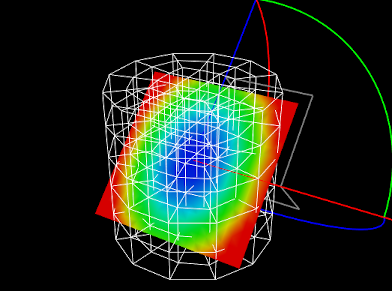
\includegraphics[]{images/ScalarFieldVisualization}
\else
 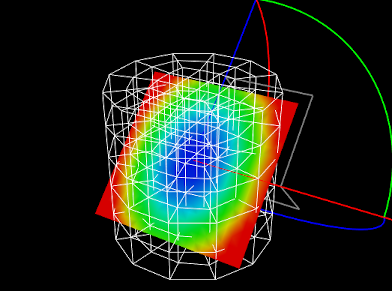
\includegraphics[width=3.75in]{images/ScalarFieldVisualization}
\fi
\end{center}
\caption{ScalarFieldVisualization model loaded into ArtiSynth.}
\label{ScalarFieldVisualization:fig}
\end{figure}

A simple application that uses a {\tt FemCutPlane} to visualize a
{\tt ScalarNodalField} is defined in
%
\begin{verbatim}
  artisynth.demos.tutorial.ScalarFieldVisualization
\end{verbatim}
%
The {\tt build()} method for this is shown below:
\lstset{numbers=left}
\iflatexml
%% Hack: latexml lstinputlisting doesn't handle firstline correctly
\lstset{firstnumber={-22}}
\lstinputlisting[firstline=1,lastline=56]{../../src/artisynth/demos/tutorial/ScalarFieldVisualization.java}
\lstset{firstnumber={1}}
\else
\lstinputlisting[firstline=24,lastline=79]{../../src/artisynth/demos/tutorial/ScalarFieldVisualization.java}
\fi
\lstset{numbers=none}
%
After first creating a {\tt MechModel} (lines 2-3), a cylindrical
hexahedral FEM model is created to contain the field, with its top
nodes fixed to allow it to deform under gravity (lines 13-17). A {\tt
ScalarNodalField} is then defined for this FEM, where the value at
each node is set to $r^2$, with $r$ being the radial distance from the
node to the FEM's central axis (lines 21-27).

To visualize the field, a {\tt FemCutPlane} is created with its pose
set to align it with the $z$-$x$ plane and then added to the FEM model
(lines 31-33). The field's visualization is then set to {\tt SURFACE}
and the cut plane is added to it as a render mesh (lines 36-37).  At
lines 40-44, a control panel is created to allow interactive
adjustment of the field's {\sf visualization}, {\sf renderRange}, and
{\sf colorMap} properties. Finally, render properties are set: the FEM
line color (used to render element edges) is set to blue-gray (line
48); the cut plane's surface rendering is set to {\tt None} to avoid
interfering with the field rendering, and axis rendering is enabled to
make the field visible and selectable even if it doesn't intersect the
FEM (lines 51-53); and, for {\tt POINT} visualization, the field is
set to render points as spheres with a radius of $0.02$ (line 55).

To run this example in ArtiSynth, select {\sf All demos > tutorial >
ScalarFieldVisualization} from the {\sf Models} menu. Users can employ
the control panel to adjust the visualization, the render range, and
the color map. When {\tt SURFACE} visualization is selected, the field
will be rendered onto the FEM/plane intersection defined by the cut
plane. Simulating the model will cause the FEM to deform, deforming
this intersection with it. Clicking on the intersection surface or the
cut plane axes will cause the cut plane to be selected. Its pose can
then be adjusted using the GUI transformer tools (see ``Model
Manipulation'' in the \artisynthManual{uiguide}{ArtiSynth User
Interface Guide}), as shown in
Figure \ref{ScalarFieldVisualization:fig}.

\begin{sideblock}
When the {\sf updating} property of the render range is set to {\tt
AUTO\_FIT}, the range will be automatically set to the range of values
in the field, and {\it not} the values evaluated over the render
surface. The latter may exceed the former due to extrapolation when
the surface extends outside of the FEM, in which case the
visualization will appear to saturate. While this is not generally a
concern because FEM field values are unreliable outside of the FEM,
one can override this effect by setting the {\sf updating} property to
{\tt FIXED} and setting the range interval manually.
\end{sideblock}

\subsection{Examples: Visualizing other fields}
\label{OtherFieldVisualization:sec}

\begin{figure}[h]
\begin{center}
\begin{tabular}{cc}
\iflatexml
 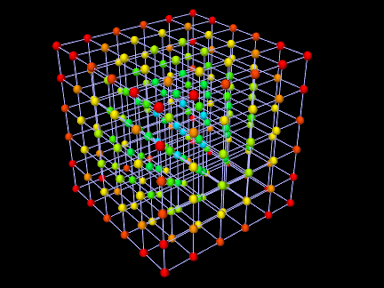
\includegraphics[]{images/ScalarNodalFieldDemo}
 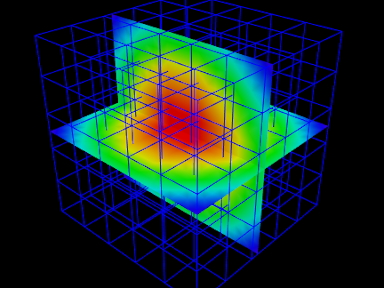
\includegraphics[]{images/ScalarGridFieldDemo}
\else
 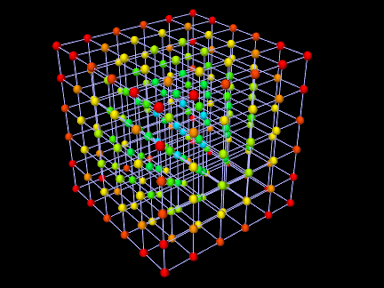
\includegraphics[width=3.25in]{images/ScalarNodalFieldDemo}
 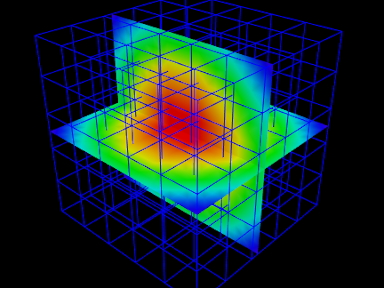
\includegraphics[width=3.25in]{images/ScalarGridFieldDemo}
\fi
\end{tabular}
\end{center}
\caption{Left: {\tt ScalarNodalFieldDemo} with {\tt POINT} visualization.
Right: {\tt ScalarGridFieldDemo} with {\tt SURFACE} visualization on
two perpendicular meshes.}
\label{OtherFields1:fig}
\end{figure}

Numerous examples exist for creating and visualizing other field types:
%
\begin{verbatim}
  artisynth.demos.fem.ScalarNodalFieldDemo  
  artisynth.demos.fem.ScalarElementFieldDemo  
  artisynth.demos.fem.ScalarSubElemFieldDemo
  artisynth.demos.fem.VertexNodalFieldDemo  
  artisynth.demos.fem.VertexElementFieldDemo  
  artisynth.demos.fem.VertexSubElemFieldDemo

  artisynth.demos.mech.ScalarVertexFieldDemo
  artisynth.demos.mech.ScalarFaceFieldDemo
  artisynth.demos.mech.ScalarGridFieldDemo
  artisynth.demos.mech.VertexVertexFieldDemo
  artisynth.demos.mech.VertexFaceFieldDemo
  artisynth.demos.mech.VertexGridFieldDemo
\end{verbatim}

Illustrations of some of these are shown in
Figures \ref{OtherFields1:fig}, \ref{OtherFields2:fig},
and \ref{OtherFields3:fig},

\begin{figure}[h]
\begin{center}
\begin{tabular}{cc}
\iflatexml
 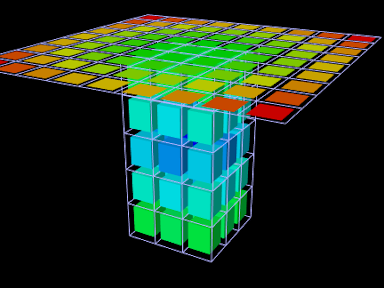
\includegraphics[]{images/ScalarElementFieldDemo}
 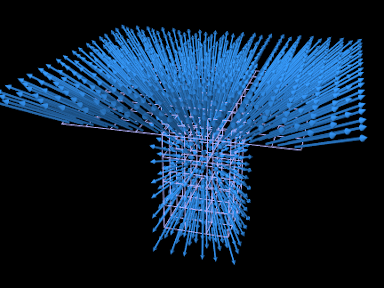
\includegraphics[]{images/VectorSubElemFieldDemo}
\else
 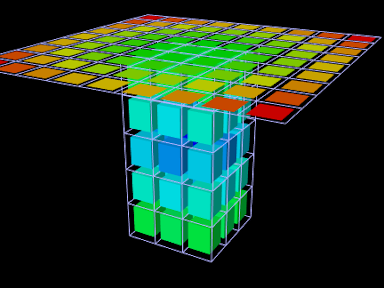
\includegraphics[width=3.25in]{images/ScalarElementFieldDemo}
 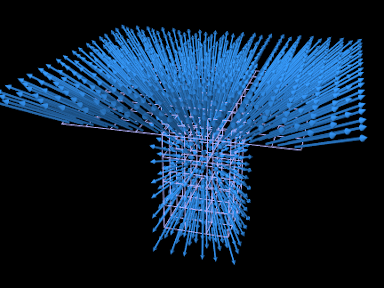
\includegraphics[width=3.25in]{images/VectorSubElemFieldDemo}
\fi
\end{tabular}
\end{center}
\caption{Left: {\tt ScalarElementFieldDemo} with {\tt ELEMENT}
visualization.
Right: {\tt VectorSubElemFieldDemo} showing vectors in blue.}
\label{OtherFields2:fig}
\end{figure}

\begin{figure}[h]
\begin{center}
\begin{tabular}{cc}
\iflatexml
 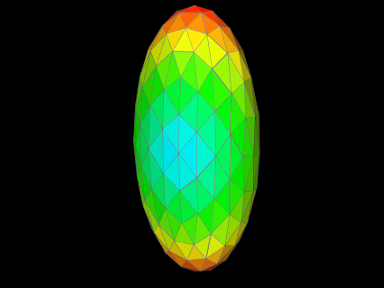
\includegraphics[]{images/ScalarFaceFieldDemo}
 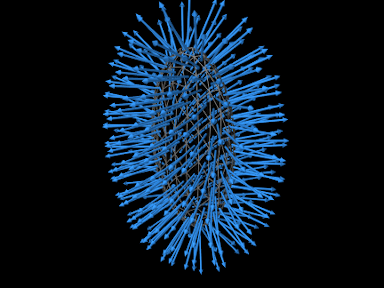
\includegraphics[]{images/VectorFaceFieldDemo}
\else
 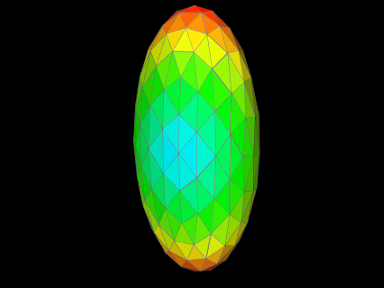
\includegraphics[width=3.25in]{images/ScalarFaceFieldDemo}
 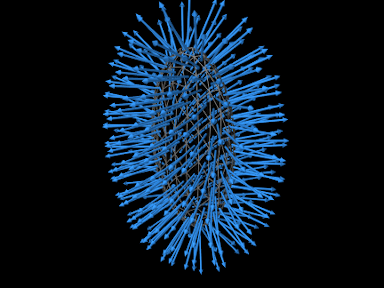
\includegraphics[width=3.25in]{images/VectorFaceFieldDemo}
\fi
\end{tabular}
\end{center}
\caption{Left: {\tt ScalarFaceFieldDemo} with {\tt FACE}
visualization.  Right: {\tt VectorFaceFieldDemo} showing vectors in
blue.}
\label{OtherFields3:fig}

\end{figure}

\ifdefined\maindoc
\else
\end{document}
\fi
